%************************************************
\chapter{Introduction}
\label{chapter:introduction}
%************************************************

In this dissertation I present the substrate for accountable layered
systems.  I have focused on building this substrate for doing
reflective thinking on a large scale in learning systems, using
{\mbox{\citeauthor{singh:2005b}'s~\citeyearpar{singh:2005b}}} example
of reflective architectures as the precedent.  My approach focuses on
a purely procedural approach that does not assume any logical search
algorithms that work behind-the-scenes without a reflective learning
focus.  This approach learns to plan in two concurrent layers of
goal-oriented optimization without increasing the computational time
complexity of a single non-reflective planning algorithm.  Learning to
plan real-time physical actions, while concurrently learning to plan
real-time planning actions.  Deliberative planning activities are
thought of reflectively in an analogous way to how the deliberative
activities think of physical activities, implying a recursive
application of the concurrent real-time reflective planning model to
itself.  The contributions of this thesis are:

\begin{itemize}
\item \emph{Emotion Machine Cognitive Architecture}: A computational
  implementation of metacognition that contains a physical simulation
  that is controlled by a deliberative physical object-level reasoning
  layer with another reflective meta-level reasoning layer that learns
  to control the first-order problem solving resources.  This is the
  result of stacking two very similar planning machines on top of one
  another, pointing toward future reflective architectures that will
  be able to recursively ``grow'' layers of reflective planning over
  any given preexisting problem solving resources.
\item \emph{Grounded Learning of Knowledge Utility}: A dependency
  tracing learning algorithm that is capable of learning both from
  ``being told'' as well as from experience, learning what types of
  knowledge are useful in different contexts, refining hypotheses for
  the utility of knowledge when they turn out to be wrong, learning by
  tracing these assumptions from expectation failures experienced
  during the execution of plans.
\item \emph{Funk Virtual Machine and Programming Language}: A
  concurrent and parallel virtual machine and lisp-like programming
  language with procedural tracing features that facilitate the
  automatic monitoring of control systems running many concurrent
  tasks.
\end{itemize}

\section{Document Overview}

The focus of the dissertation will be a description of the reflective
problem of learning-to-control.  I describe control in terms of layers
of reflective credit assignment because this simplifies understanding
the problem of learning-to-control.  Throughout this dissertation I
will use a running example of learning to accomplish goals in a simple
block building domain, similar to the Blocks World planning domain
\cite[]{winograd:1970}.
\autoref{chapter:reflectively_learning_to_control} describes my
implemented solution to the problem of reflectively learning to
control.

\section{Closed-loop Control and Learning}

There are many artificial intelligence algorithms that provide
explanations for how to accomplish goals or gather rewards in a
domain. A basic artificial intelligence system consists of three
processes: (1) perceptual data are generalized and categorized to
learn induced abstract models, (2) abstract models are used to infer
expected hypothetical states, i.e. states of future, past, or
otherwise ``hidden'' variables, (3) actions are chosen based on
considerations of different action and hypothesis dependent
inferences.  While there are many types of machine learning algorithms
that focus on this abstract 3-step closed-loop process of learning to
control, the field of metacognition \cite[]{cox_and_raja:2008} focuses
on making at least two layers of closed-loop systems. The first
closed-loop learning algorithm learns how to deal with the external
world, while the second closed-loop learning algorithm perceives the
state of the algorithm below. I see metacognition as a layering of
learning algorithms, such that the second layer algorithm learns from
perceiving the activity of the first layer and controls or modifies
this first layer. While it may be clear how to trace changes in the
perceptual inputs of layer one of the algorithm, it is less than clear
how the second layer learner should monitor the changes in the state
of the first layer learner.

\section{Reflection in Computer Science}

The term reflection is a commonly used word in computer science and
AI.  The idea is extremely simple and is a modelling contribution of
this thesis, but, because of its simplicity, it is a widely applicable
idea.  In fact, \cite{maes:1988} distinguishes over 30 different types
of \emph{computational reflection}, grounded in the computer science
literature.  The type of computational reflection that is introduced
in this dissertation is not included in Maes' overview, although the
implementation of this model is based on many of the forms of
computational reflection that Maes does describe, e.g. procedural
reflection, type reflection, frame reflection, and others.  She does
not mention the type of reflection that I am focused on in this thesis
because it was not, at the time, commonly considered computational.
The type of reflection that is modelled here is a psychological type
of reflection: the ability to think about thinking in addition to the
ground problem.  This psychological form of reflection is modelled as
a learning-to-control problem in this thesis.

\section{Learning to Plan for Successful Execution}

Dependency traces for a hypothesized successful plan creation compose
an important set of knowledge to associate with a plan for debugging
the planning process when, later, it is realized that the plan fails
to execute.
{\mbox{\autoref{figure:dependency_traces_and_tracing_bug_dependencies}}}
shows a picture of dependency traces with hypothesis creation events
being pictured as shapes on a time line.  These hypotheses have arrows
between them that represent the derivation dependencies of each
hypothesis creating decision.  The circles in the picture represent
the symbolic states of the world that are used to create hypotheses,
which are represented by squares.  If any hypothesis is used to derive
another hypothesis, these dependencies give a credit assignment path
that is able to jump back retrospectively an arbitrary distance in
time as well as between reflective layers.  Notice in the picture that
the circle on the far left is a dependency of a square block, but
these two events are not necessarily consecutive in time.  If a
hypothesis is derived from a number of other hypotheses, possibly far
in the past, and this hypothesis fails in action, each one of these
traced dependencies represents a learning opportunity.  Every
additional layer of reflective control in the model, represents
another hypothetical learning opportunity, leading to more efficient
search toward plans that succeed in execution.

\section{Finding a Bug}

The credit assignment problem arises when a bug occurs in some part of
the system.  For example, plans can fail physically to accomplish what
they have been previously hypothesized to accomplish.  There are many
knowledge dependency algorithms that work at this physical knowledge
level.  In this thesis, a layered reflective knowledge representation
is presented for propagating failures to knowledge manipulation
actions as well as physical actions.
{\mbox{\autoref{figure:dependency_traces_and_tracing_bug_dependencies}}}
represents a bug found in a planning hypothesis.  For example, the
planning hypothesis could be that some certain planning activity leads
from one type of plan to a plan that will successfully complete
execution without failing.  Failure propagates through reflective
layers of goals and distinct classes of hypotheses.  Bugs are
propagated through every reflective layer and, therefore, each
reflective layer is presented with a different learning opportunity.
\begin{figure}
\center
\begin{tabular}{c}
  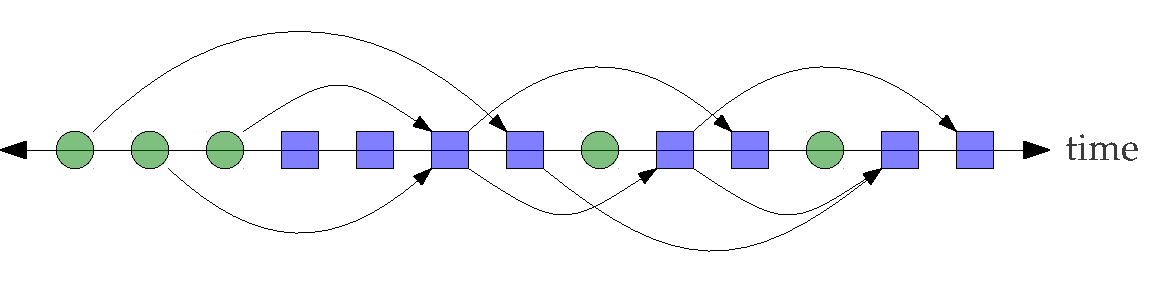
\includegraphics[width=10cm]{gfx/dependency_traces} \\
  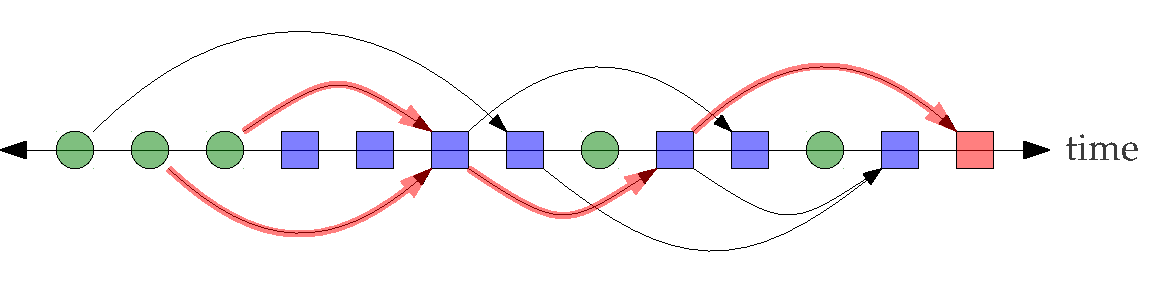
\includegraphics[width=10cm]{gfx/tracing_bug_dependencies}
\end{tabular}
\caption[Dependency traces and tracing bug dependencies.]{\emph{(Top)}
  Dependency traces, where circles are symbols, squares are
  hypotheses, and arrows are dependencies.  \emph{(Bottom)} Tracing
  bug dependencies, where the bold arrows represent the credit
  assignment path for a failure in a hypothesis, represented by the
  square on the far right.}
\label{figure:dependency_traces_and_tracing_bug_dependencies}
\end{figure}





%\section{Hypotheses and Decisions}

%let me just go through a simple example of what a decision is because this becomes very confusing very quickly if we don't ground that idea out.
%this dog looks hungry should i feed him?
%he may bite me.
%this is a basic decision, so let's say we have two options
%how do we think about modelling these two options.
%we're in a current state
%it could possibly lead to two other states
%the question is: what action should we take?
%there is a lot of complicated processing that could into making this decision, but if we just want to talk about the basic development of what a hypothesis is and how do we develop the provenance of data based on that.
%that's what i'm building this up to.
%we have to choose of all of the knowledge we have, maybe from the current state, maybe from the past, which should this decision be based on?
%that's a very complicated problem.
%generally these algorithms are focused on a dataset, so they're not required to learn those types of relationships.
%how should i weigh my relative goals into this decision?
%certain algorithms will have a clear ranking of goals, like a reinforcement learning algorithm will have basically, any time you get into an important state, it will give you an exact number, this state was worth this much.
%this state was worth ten.
%this state was worth negative ten.
%the system that i'm talking about is a little more general than that.
%it uses multiple goals.
%they can have partial orderings.
%but you have to consider, some of the may not even be directly related, so you may have to, part of this decision process could be coming up with that partial order.
%i'd like to dog to not be hungry.
%i also don't want to be bitten.
%you're defining the states of the world that you're going to pay attention to.
%what might be the results of this?
%what might be the relationships?
%what are the relationships now that might help us to make this decision?
%for example, the properties of the dog that we might be paying attention to.
%let's say, there is a hunger for the dog.
%he looks hungry or he looks full.
%these are all things that we're perceiving to make this decision.
%the dog has a color, a breed, it could be barking or not, its going to tell us whether or not the dog is going to bite us basically.
%how do we develop a hypothesis?
%we may have multiple sets of training data.
%this may be our first example.
%we want to take the current situation and we want to make a prediction.
%what kind of hypotheses could we use?
%what does a hypothesis even look like?
%if we feed the dog, there are a bunch of things that might happen.
%he could fall asleep.
%he could continue to be hungry.
%here's a set of examples.
%imagine that we're feeding these examples into the algorithm 1 through 4 on the lefthand side there.
%there are a number of properties that we could then categorize into, for each of these numbered examples we could predict the category on the right.
%we're trying to predict whether or not our hand was bitten given the features on the dog.
%it's basically a function approximation algorithm that we're trying to develop as a hypothesis for this state space.
%
%minsky: mark twain had advice about buying a stock.
%if it goes up sell it.
%if it goes down don't but it.
%
%bo: i think there's a loop in that causal chain.
%i've tried to avoid those.
%
%what's the point?
%why are we talking about this?
%goals!
%because we have goals.
%there are good parts of the world
%there are bad parts of the world
%we want to know how to get to the good parts and avoid the bad parts
%we have avoidances
%we have goals
%we have states of the world
%these might be partial states of the world that we want to pursue or avoid
%deciding on an action depends on weighing these considerations
%what is the state of the world going to be?
%which parts is it going to contain?
%to make this categorization, here's an example.
%very simple algorithm is relatively efficient for doing what it does for getting conjunctions of features as hypotheses for what might predict a category.
%for example, this line here, the first two question marks with "pitbull yes" means "if the statement contains pitbull and it contains that the pitbull is barking then it is categorized as this type of category."
%you can imagine the more general hypothesis is that every dog is going to bite me
%that's all question marks, any of these features match.
%the most specific hypothesis is that none of these features could possibly match
%no matter what feature you tell me its always going to not bite me
%it is a perfectly safe dog.
%these are one example and then two ends of the range of this hypothesis space.
%so, hypothesis h of x is a function that takes state x and predicts whether or not it is an instance of a category.
%what are all of the possible hypotheses that we could learn?
%this is called the inductive bias of the algorithm.
%this is the assumption that we come to the state space with a certain language that we're going to describe our hypothesis within.
%in general this could be a very complicated language.
%in this case its very simple.
%it is just a conjunction of features.
%it helps us to think of these features.
%i'm just going to go over these quickly because this is not fundamental to the theory, but this is just showing that we can efficiently implement a search over the entire hypothesis space.
%we can use a general to specific concept ordering.
%if we consider one concept always predicts that this is a positive category whenever this other concept predicts that its a positive category, then we can say that the hypothesis that predicts it more often is more general than the hypothesis that predicts it less often.
%h 0f j would be the hypothesis that predicts it more often, h of k would be the less often predictor, so there an implication reelationship between every positive instance of h of k to h of j.
%
%making decisions given hypotheses.
%we have collections of these hypotheses that we can efficiently keep track of.
%given training input into this algorithm.
%this is called the version space learning algorithm, which i'm not going into the details of because it isn't important.
%we have hypotheses represented.
%we have collections of every single hypothesis that matches the given training input
%we can efficiently keep track of that
%given a new training instance we can run it through this decision machine to predict what the output is going to be
%when all of our hypotheses agree, we know that we can be confident in our prediction
%when the hypotheses disagree, this is given the assumptions of the version space learning algorithm, which means that the hypothesis that we're looking for is actually in the hypothesis space that we've chosen and things like that.
%if all of the hypotheses agree, then we know that this is the right answer.
%the hypothesis is in that space and it would also agree.
%when the hypotheses disagree it becomes a lot more interesting.
%so, how do we make decisions?
%it could go one of two possible ways depending on if our hypothesis is in one set or the other, but we still act
%we make some kind of assumption there.
%there are probabilistic formulations of this for decision theory that says "all of my hypotheses are equally likely"
%you need a prior on your hypothesis space that gives some kind of weighting on these things so that you can make a decision
%there are 10 hypotheses that say yes there are 5 that say no, given that they're all equally probable, i'm going to take the one that says yes.
%you can make those decisions.
%you can apply those assumptions to this algorithm.
%
%in any case, you do have to make a decision, if you do make the decision which is useful, then you can keep track of that decision's knowledge.
%yes, i'm going to imagine this state of the world.
%you can associate with that knowledge the hypotheses used to generate it.
%you can even imagine going both ways.
%if you consider that both of these are possible outcomes, you can imagine both possible states given the hypotheses that derive them.
%we understand decision making.
%the definition of the hypothesis is relatively clear.
%the tracing the provenance of data is relatively clear.
%
%the causal tracing of processes.
%this is the low level computer science graphic of how you would trace a process.
%we have low level commands or events that we are told to execute.
%this is a normal AI program that is just running without reflection.
%we can imagine a loop being hardcoded into this algorithm, a sequence of events that has pointers back to loop.
%there's the process sitting there in memory.
%we can run this process.
%we can take a virtual machine.
%this is loading the process into the execution register of the machine.
%it starts running.
%that's all the execution register knows how to do.
%it just interprets and starts running.
%this is what a normal AI system will do.
%you load the program into the processor and it executes the program.
%what we've added to this is the creation of semantic events.
%when something important happens in the process below, we create a sequence of semantic events.
%things that might be important to keep track of.
%this function is just beginning its an important function so maybe you should know about that.
%that function has exited successfully.
%there were not bugs in it or i wouldn't have gotten here.
%keeping track of all of these kinds of events can give us knowledge to reflect over the process.
%its a basic low level computer science, computational reflection.
%i'm going to distinguish that from the psychological word of reflection which i'm going to use to refer to controlling the deliberative process.
%we keep track of these semantic events, which then we can recognize.
%oh this pattern looks like this function is entering.
%this function looks like this function is executing.
%we can then have responses that happen in parallel to the basic running process.
%there is an efficiency thing that we can talk about here.
%the tracing of the events require a constant time slowdown.
%algorithmically, that isn't a slowdown, theoretically, its big O notation.
%this algorithm is running the same speed and now we've added computational reflection to it.
%
%gjs: what is this diagram showing?
%i'm confused.
%
%bo: there is a list of.  we can think of these as low level instructions to a machine, like bytecode operations.
%
%gjs: yes.
%
%bo: these bytecodes have a jump from the C to the W there.
%
%gjs: right.
%
%bo: this virtual machine is like a thread.
%
%gjs: yes.
%
%bo: you can load this program in to have the thread start running it.
%then on the top we can keep track of a trace of semantic events.
%
%gjs: i'm confused about these top things that look like a sliding R on a little device I could carry around.
%
%bo: this is meant to be a physical analogy.
%it's kind of like chemistry with the dna.
%
%gjs: i'm trying to figure out what its an analogy to.
%what are you trying to actually
%
%bo: right.  let me describe the analogy and then i'll describe how its implemented.
%the analogy is that we have dna.
%we have transcriptase running along the rna
%and its creating amino acids that end up folding into proteins.
%what this end up doing is it reads along this chain and its creating this string, which is basically, these are the amino acid codons that i want to be attaching to me.
%
%gjs: is the string the one in the purple?
%
%bo: the string is the one in the purple.
%
%gjs: yes, okay.
%
%bo: these are the codons that i want to attach.
%these basically represent the amino acid binding.
%
%gjs: these things on top are patterns.
%is that what they are?
%
%bo: these are patterns.
%
%gjs: they match something?
%
%bo: right.
%
%gjs: ah.  thank you.
%
%bo: they're meant to be floating around and then they float down and bind to the string.
%
%gjs: okay.
%
%bo: this is the physical analogy.
%how that's implemented is you have a stream with multiple listeners each one recognizing a pattern.
%
%gjs: fine.
%
%bo: i use the physical analogy because there's parallel processing.
%you can imagine the basic transcriptase running along the molecule without worrying about slowing down the other molecules around it in their physical simulation.
%we can have responses that are other processes that immediately begin running concurrently.













